\chapter{Experimenty}

V tejto kapitole popisujeme vstupné dáta, nastavenia infraštruktúry nabíjacej siete, ceny nabíjania v čase, ktoré používame v experimentoch.
 Spomíname aj využité technológie, vďaka ktorým môžeme porovnať naše riešenie s doterajšími riešeniami. Niektoré technológie (\ref{technolgie:acnportal}) sme použíli v nami implemenotaných algoritmoch.

% v tejto kapitole treba uviest vsetkky experimenty, ktore ukazuju moj vysledok
% aj vstupne a vystupne data
\section{Ukážka vstupných dát ACN-Data}
\begin{figure}[H]
    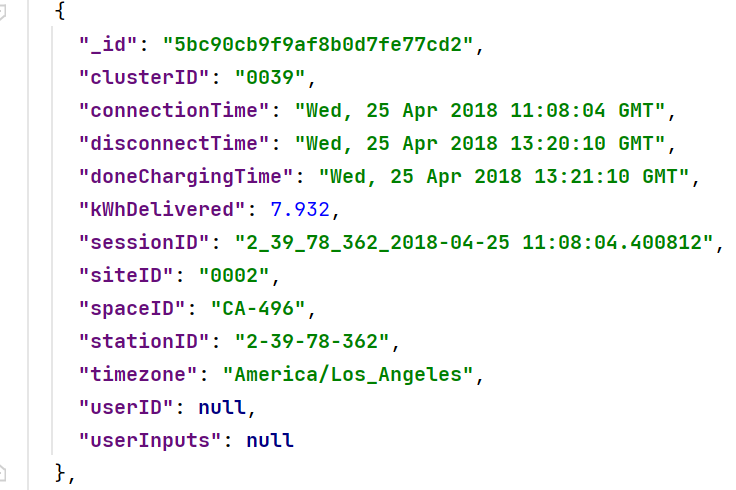
\includegraphics[width=0.8\textwidth]{images/acndata.png}
    \centering
    \caption[Ukážka vstupných dát ACN-Data]{Vstupné dáta z nabíjania jedného elektromobilu, ktorý prišiel na nabíjaciu stanicu 25. Apríla 2018. Zdroj: \cite{websiteacndata2023}.}
    \label{acndata:obr}
    \end{figure}
Obrázok vstupných dát \ref{acndata:obr} obsahuje viacero parametrov, ktoré používateľ musí zadať (napr kWhDelivered), aby mohol nabíjať svoj elektromobil na jednej staníc Caltech, JPL alebo Office001. Iné nabíjacie stanice používajú odlišné vstupné dáta, uvádza sa v \cite{lee2021adaptivephd}.

\section{Využité technológie}
V tejto sekcii spomíname technológie, na ktorých spočíva naša implementácia. Balíky popisujeme hlavne na základe informácií uvedených v ich README súboroch a na základe článku \cite{lee2021acnsim}. Podrobný návod, ako vytvoriť algoritmy na základe nasledujúcich balíkov sa nachádza v \cite{lee2021acnsim}.
\label{vychodiska:technologicke}

% TODO: nabijat len 8 amperov? skontrolovat!!!

\subsection{Balík acnportal.}
\label{technolgie:acnportal}

% \subsection{Balík acnportal.}
% \subsection{Balík acnportal}
Balík acnportal je predovšetkým určený na zrýchlenie výskumu nabíjania veľkého množstva elektrických áut. Balík acnportal umožnuje zrýchlenie výskumu pomocou výskumných nástrojov vyvinutých v Caltechu. 
% Balík acnportal pozostáva z viacerých výskumných nástrojov vyvynutých v Caltechu, aby sa zrýchlil výskum nabíjania veľkého množstva elektrických vozidiel v nabíjacej stanici.
%  Každý záznam nabíjania elektrických vozidiel obsahuje jeho príchod, odchod a požadovanú energiu. Balík acnportal sa nachádza v \cite{acnportalrepository}. 
 
 Balík acnportal pozostáva z viacerých komponentov:

\begin{enumerate}
    \item \textbf{ACN-Data}: Dáta získané z nabíjacích staníc pre elektromobily, konkrétne zo staníc Caltech, JPL a Office001. 
    Vodiči elektrických vozidiel musia cez mobilnú aplikáciu zadať oskenovaný QR kód nabíjačky a potom zadať približný čas odchodu a množstvo požadovanej energie. 
    %Ak vodič neuvedie informácie cez mobilnú aplikáciu, nabíjačka bude nabíjať len 8 ampérov a ak ani po 15 minútach vodič neuvedie informácie, tak nabíjačka prestane nabíjať.  
    Dáta získané od vodičov elektrických vozidiel, a aj dáta slúžiace na konfiguráciu nabíjacej stanice sú uložené v relačnej databáze. 
    % overit predchadzajucu vetu
    Vďaka tejto úložnej vrstve vieme vytvárať vizualizácie pre vodičov elektrických vozidiel a pre sieťových operátorov. 
    Ide hlavne o vizualizáciu stavu systému pre sieťových operátorov a stav nabíjania elektromobilov pre vodičov elektromobilov.
    \item \textbf{ACN-Sim}: ACN-Sim je simulátor používaný na testovanie a overovanie funkcionality algoritmov a systémov. Simulátor zabezpečuje realistické prostredie na overovanie funkcionality algoritmov, hlavne pre výskumníkov, ktorý nemajú prístup k reálnym nabíjacím systémom pre nabíjanie elektrických vozidiel.
    \item \textbf{ACN-Live}: ACN-Live je hardvér, na ktorom bežia online plánovacie algoritmy na nabíjanie elektrických vozidiel v reálnom čase. Keďže má rovnaké rozhranie ako simulátor ACN-Sim, tak vieme testovať algoritmy implementované v ACN-Sim bez zmeny kódu. \cite{lee2021acnsim, lee2020adaptive}
\end{enumerate}

\begin{figure}[H]
    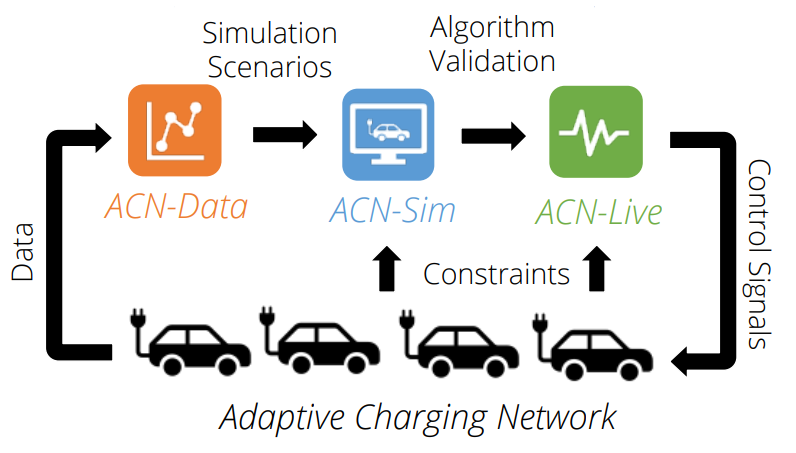
\includegraphics[width=0.8\textwidth]{images/acn_research_portal_pic.png}
    \centering
    \caption[Schéma acnportal.]{Schéma acnportal. Zdroj obrázka je \cite{lee2021acnsim}.}.
    \label{acn:obr}
    \end{figure}
Obrázok \ref{acn:obr} ilustruje interakciu medzi komponentami acnportal. Dáta o nabíjaní získava komponent ACN-Data. O obmedzenia siete a validáciu algoritmov sa stará komponent ACN-Sim. V komponente ACN-Live sa uvádzajú algoritmy z komponentu ACN-Sim do prevádzky. Na takú operáciu netreba meniť kód, lebo ACN-Sim a ACN-Live fungujú cez rovnaké rozhranie. \cite{lee2021acnsim,lee2021adaptivephd}

%TODO: overit vsetky napisane udaje, musi to sediet!




\subsection{Architektúra simulátora ACN-Sim}

\begin{figure}[H]
    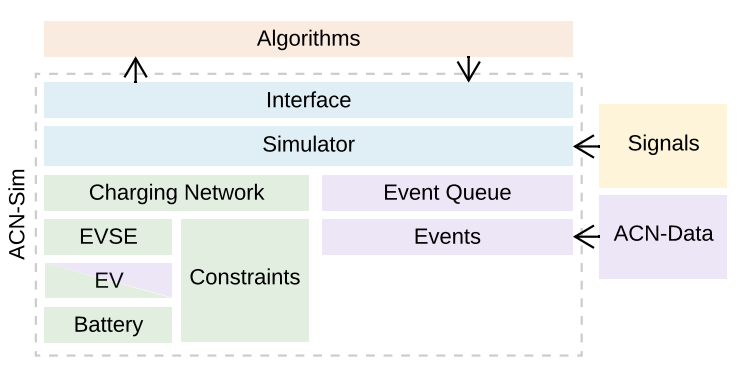
\includegraphics[width=0.8\textwidth]{images/acn_architecture.png}
    \centering
    \caption[Architektúra simulátora ACN-Sim.]{Architektúra simulátora ACN-Sim. Obrázok pochádza z článku \cite{lee2021acnsim}.}
    \label{architectureacnsim+:obr2}
    \end{figure}
Obrázok \ref{architectureacnsim+:obr2} popisuje architektúru simulátora ACN-Sim. Simulátor ACN-Sim má modulárnu, objektovo orientovanú architektúru. Pod každou krabicou v obrázku \ref{architectureacnsim+:obr2} chápeme základnú triedu, od ktorej môžu dediť nové triedy. Tieto nové triedy môžu napríklad obsahovať nové funkcie.  


% TODO:nepresne napisane
Simulátor ACN-Sim obsahuje udalosti popisujúce príchod a odchod elektromobilov. Každá udalosť obsahuje informáciu, v ktorom časovom kroku behu simulátora sa má vykonať. V každom časovom kroku behu simulátora sa vykonávajú udalosti v predchádzajúcom časovom kroku alebo udalosti v aktuálnom časovom kroku. Po každej vykonanej udalosti sa spustí plánovací algoritmus a stav infraštruktúry sa aktualizuje. \cite{lee2021acnsim}


% \begin{figure}[H]
%     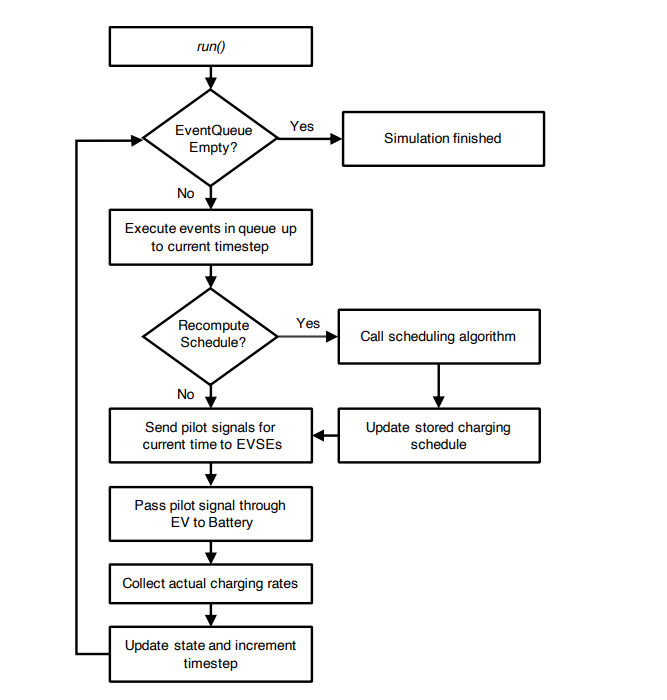
\includegraphics[width=0.8\textwidth]{images/simulator_run.png}
%     \centering
%     \caption[Vývojový diagram funkcie run() simulátora ACN-Sim.]{Vývojový diagram funkcie run() simulátora ACN-Sim. Obrázok pochádza z článku \cite{lee2021acnsim}.}
%     \label{architectureacnsim+:obr2}
%     \end{figure}

% \UNFIN

% nám pomáha pochopiť štruktúru a interakcie jednotlivých častí systému, aby sme vedeli implementovať vlastné algoritmy.


% \subsection{Interakcia medzi spotrebitelmi a smart grid}


%vsetky baliky sa zacinaju malym pismenom a su oddelene pomlckami

% TODO: blizsie popisat z coho pozostava ten balik!!!!
% namiesto repozitar balik napriklad!!
\subsection{Balík adacharge.}
% \subsection{Balík Adacharge}


% TODO:prepisat prva veta je zla MPC samotny to neriesi ale metody v mpc
Balík adacharge obsahuje kontrolný algoritmus MPC, ktorý je schopný riešiť viacero optimalizačných problémov v rámci plánovania nabíjania elektromobilov. Tento MPC algoritmus rieši aj problém, ktorý my riešime, a to problém pridelenia maximálnej energie elektromobilom pri zachovaní obmedzení infraštruktúry pomocou konvexnej optimalizácie. Podrobnejší popis a zdrojový kód balíka Adacharge sa nachádza v \cite{adachargerepository}.
% aj zaroven obmienat
\subsection{Balík acnportal-experiments.}
Účelom balíka acnportal-experiments je zdieľanie experimentov, ktoré pomocou balíka acnportal riešia rôzne vedecké otázky.
% Balík acnportal-experiment obsahuje experimenty, ktoré využívajú balík acnportal. 
% Tieto experimenty následne vedia zodpovedať výskumné otázky. 

Pre tvorbu nových experimentov, ktoré riešia náš problém sú podstatné experimenty 1.2 a 2.1. Tieto experimenty využívajú viacero plánovacích algoritmov a konfigurácii siete. Krátky popis experimentov:
\begin{enumerate}
    \item Experiment 1.2: Cieľom experimentu je porovnať viacero konfigurácii infraštruktúry siete a zároveň plánovacie algoritmy. Tento experiment poukazuje na výhody smart sietí. Jednou z výhod smart sietí je, že vedia riešiť problém dodania maximálneho množstva energie pri zachovaní obmedzení infraštruktúry siete.
    \item Experiment 2.1: Cieľom experimentu je porovnať výkonnosť týchto plánovacích algoritmov:  round robin,  earliest deadline first, least laxity first. Jedným z výsledkov experimentu je koľko percent požadovanej energie dodá elektromobilom každý algoritmus.
\end{enumerate}
%experiment 2.2 mozno pridat ale netyka sa toho co my riesime, riesi vykonnost planovacich algoritmov pri zmene modelu baterie atd


\subsection{Balík stable-baselines3.}
\label{technologie:sb3}

Balík stable-baselines3 vytvorili za účelom implementovania viacerých spoľahlivých algoritmov učenia posilňovaním (vývojári otestovali výkonnosť všetkých algoritmov). My používame algoritmus SAC z balíka stable-baselines3 na učenie a testovanie algoritmu [odkaz...].  Balík stable-baselines3 obsahuje podrobnú dokumentáciu a aj obsiahlu funkcionalitu.




Podrobnejší popis a výsledky experimentov vieme nájsť v \cite{acnportalexperimentsrepository}.

%TODO: pojmy ako transformer vysvetlit alebo odstranit
%TODO: mozno pridat aj ten 3. experiment?
%TODO: pisat tie mena algoritmov jednotne
% \UNFIN

% \section{Aplikovateľnosť smart charging algoritmov.}

% Mnoho zaujímavých algoritmov z literatúry sa nedá využiť priamo v praxi. Hlavným dôvodom prečo sa nedajú aplikovať v praxi je poďla \cite{lee2021adaptivephd} to, že majú predpoklady, ktoré v praxi nefungujú alebo im chýba schopnosť splniť praktické obmedzenia a aj ciele.

% Uvádzame list vlastností smart changing algoritmu spomen , ktorý môže byť aplikovateľný v praxi:

% \begin{enumerate}
%     \item Algoritmy musia brať do úvahy používateľské vstupy ako napríklad čas odchodu a množstvo požadovanej energie.
%     \item Algoritmy musia vyriešiť jednoducho problém s viacerými cieľmi.
%     \item Algoritmy musia vedieť pracovať s obmedzeniami v niekoľkoúrovňovej nevyváženej infraštruktúry.
%     \item Výstup algoritmov (plán nabíjania) musí spĺňať aspoň jednu z týchto vlastností: plynulé nabíjanie alebo spravodlivé zdielanie kapacity medzi elektromobilmy.
%     \item Algoritmy musia byť odolné voči neistote v budúcich príchodoch elektromobilov. 
%     \item Algoritmy musia vedieť narábať s diskrétnymi bodmi pre pilotové signály.
%     \item Algoritmy musia mať schopnosť si nárokovať nevyužitú kapacitu v prípade, keď elektromobili nevyužívajú alokovaný pilotový signál. 
% \end{enumerate}

% Algoritmus, ktorý všetky tieto podmienky spĺňa sa nazýva Adaptive Scheduling  Algorithm (ASA). Podrobnejší popis, prečo tieto podmienky tento algoritmus spĺňa a aj list podmienok z ktorého sme čerpali sa nachádza v
% \cite{lee2021adaptivephd}.

% acnportalexperimentsrepository

% \subsection{Balík Acnportal-experiments}


% V tejto sekcii spomíname knižnice, frameworky a ďalšie technológie, ktoré sme pri implementácii použili.

% \subsection{Knižnica numpy}
% \label{ss:vych:techvych:numpy}
% Knižnica numpy rozširuje možnosti v oblasti práce s poľami. 
% V knižnici numpy sú 2 hlavné objekty: ndarray a ufunc. Pomocou objektu ndarray vieme definovať N-dimenzionálne pole a pomocou ufunc vieme definovať matematické funkcie. Každé pole objektu ndarray obsahuje homogénnu kolekciu prvkov.
% % Tie sa v štruktúre s bežnými poľami neodlišujú, to znamená že prvý prvok poľa má index 0 a posledný $n-1$, kde $n$ je dlžka poľa. 
% Naviac vieme pomocou knižnice numpy zjednodušiť zložité cykly pomocou operacií numpy.dot alebo numpy.outer, čo značne zlepšuje časovú zložitosť programu. \cite{oliphant2006guide}


% \subsection{Knižnica scipy}
% \label{ss:vych:techvych:scipy}

% % \subsection{Knižnica matplotib}
% % \label{ss:chapter:section:subsection}

% \subsection{Knižnica pytorch}
% \label{ss:vych
% :techvych:torch}
% Knižnica pytorch bola založená facebookovou skupinou študujúcu umelú inteligenciu. Hlavným cieľom vývoja tejto knižnice bolo zjednodušiť tvorbu a vývoj modelov. Knižnica pytorch je založená na knižnici torch a používa sa v programovacom jazyku Python.
% Pytorch je knižnica určená na písanie dynamických modelov. Z toho dôvodu sa často používa na veľké konštrukcie hlbokého učenia. \cite{mishra2019pytorch}
% Tu je nejaký text.

% \subsubsection{Subsubsection}

% Tu je nejaký text.

% \paragraph{Paragraph}

% Tu je nejaký text.

% \subparagraph{Subparagraph}

% Tu je nejaký text.

\section{Konfigurácia  a obmedzenia nabíjacích sietí}
\label{vych:konfaobmedzenia}

V tejto sekcii uvádzame jednotlivé konfigurácie a obmedzenia nabíjacích sietí, na ktorých navrhujeme a overujeme model agregátora flexibility. Vysvetľujeme postupne rôzne typy nabíjania, obmedzenia sietí atď.

% \section{Teoretické východiská.}

% Definície a vety a notácia, ktoré uvádzame ak nie je bližšie špecifikovaný zdroj, tak pochádzajú z článkov~\cite{Li_2021} a~\cite{10.1145/3307772.3328313}.
% zo statnej stranky commonwealth of messetsusec
\subsection{Typy nabíjania.}
% \subsection{Typy nabíjania}

% TODO:ako vieme kedy nabijame ac level1 a kedy ac level2 v acnportal?
Všetky experimenty, ktoré vykonávame používajú nabíjanie typu AC level 1 alebo nabíjanie typu AC level 2. Nabíjanie AC level 1 je predovšetkým určené pre vlastníkov elektrických vozidiel, ktorí ich chcú nabíjať dlhodobo (napríklad cez noc). 
Rýchlosť nabíjania typu AC level 1 je 1.4 kWh až do 1.9 kWh energie. Nabíjanie typu AC level 1 dokáže úplne nabiť batériu elektrického vozidla v rozmedzí od 8 do 20 hodín (v závislosti od kapacity batérie a typu batérie elektrického vozidla).
% Kapacita nabíjacieho kábla je od 110 až do 120 voltov.


Typ nabíjania AC level 2 je rýchlejší typ nabíjania ako AC level 1. Rýchlosť nabíjania pri AC level 2 je od 2.5 kWh do 19.2 kWh. Počas dňa môže viacero spotrebiteľov nabíjať vďaka takejto rýchlosti nabíjania. 

Pri takejto rýchlosti nabíjania elektrických vozidiel sa môže vystriedať pri nabíjaní počas dňa viacero spotrebiteľov. Nevýhodou typu nabíjania AC level 2 je, že vyžaduje väčšie náklady na inštaláciu.
% Kapacita nabíjacieho kábla pri AC level 2 je buď 208 alebo 240 voltov.
\cite{charginglevelsumini, websitecharginglevels2023}

\begin{figure}[H]
    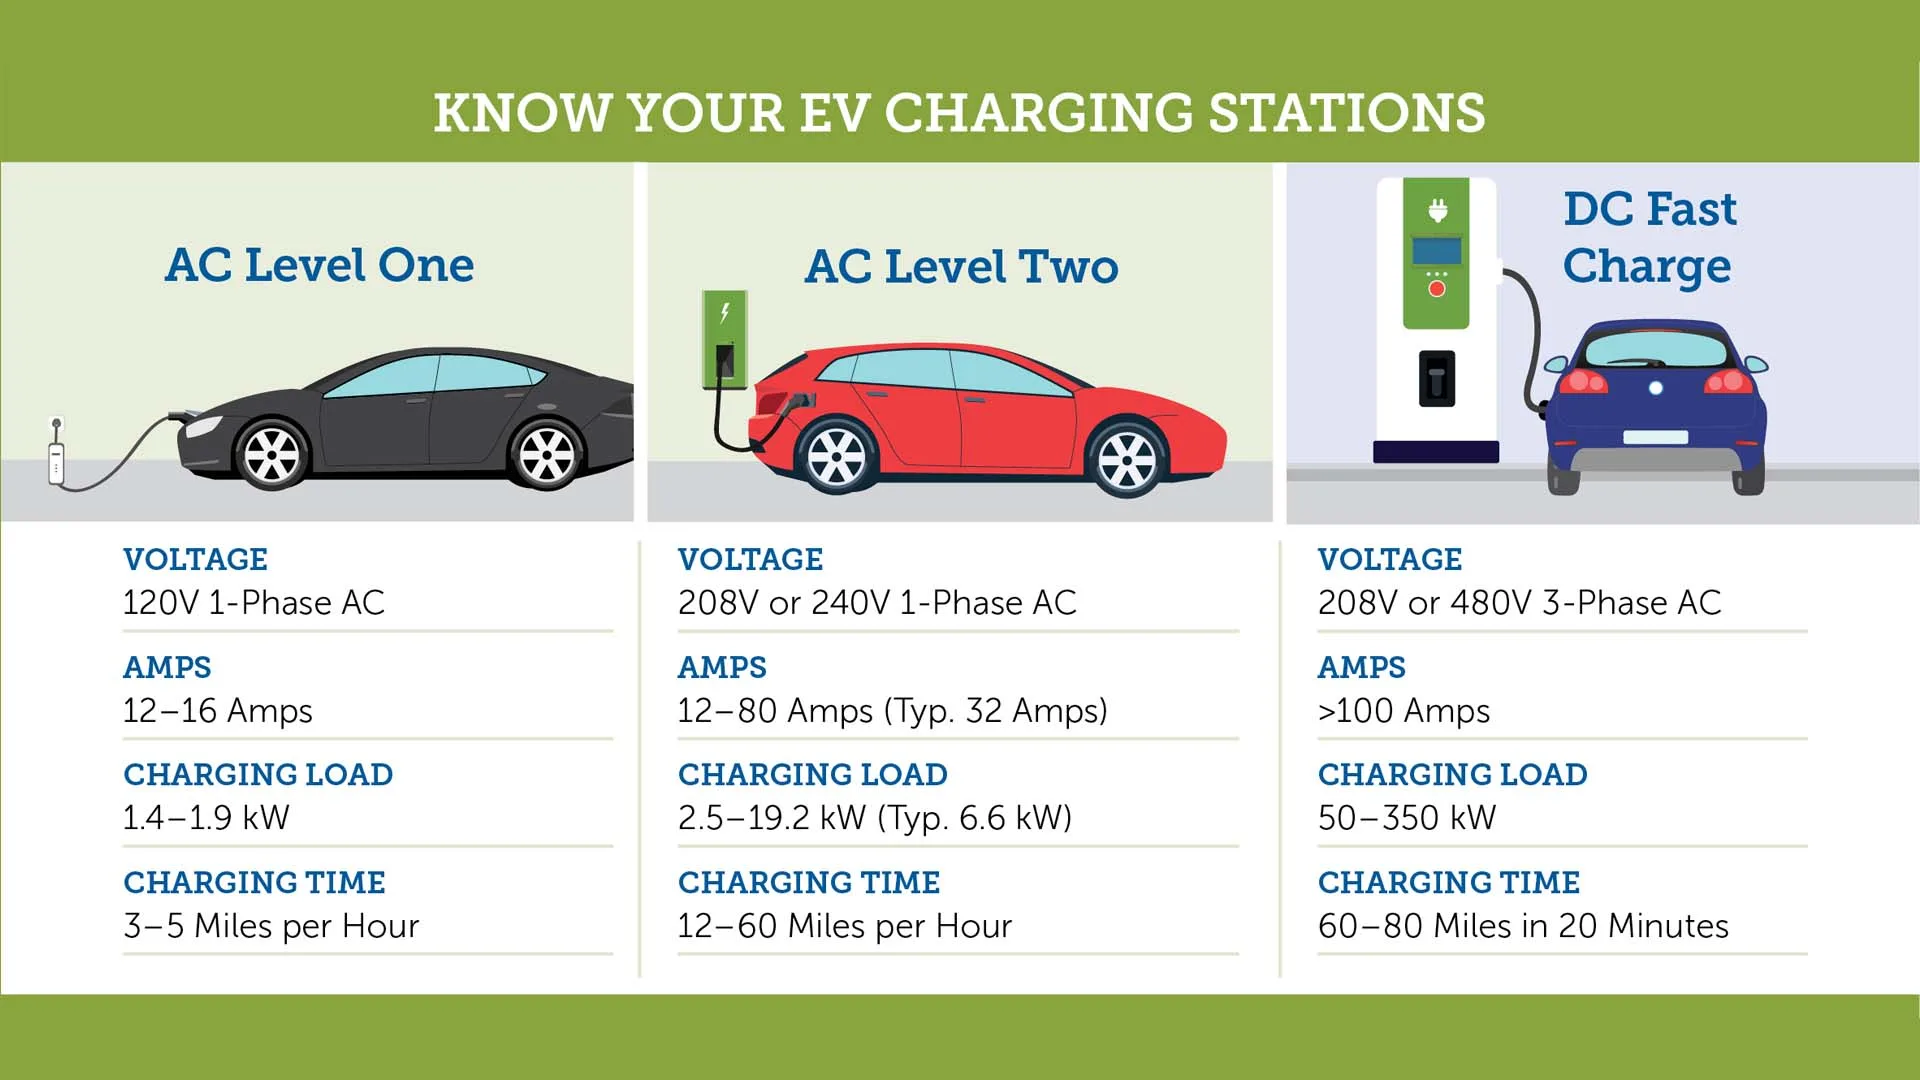
\includegraphics[width=1\textwidth]{images/EVCharger-Levels-jpg.png}
    \centering
    \caption[Typy nabíjania elektromobilov]{Všetky dnešné typy nabíjania elektromobilov s príslušnými údajmi o rýchlosti nabíjania a kapacite kábla. Zdroj obrázka: \cite{websitecharginglevels2023}.}
    \label{typynabijania:obr}
    \end{figure}
% TODO: ak bude mozne najst obrazok ohladom levelov nabijania z literatury (zatial som nenasiel)

% ale malo by to byt ok 
% 1. dalsi zdroj co ma rovnako https://craigheadelectric.coop/electric-vehicle-charging-101/
% 2. dalsi zdroj co to ma rovnako https://www.linncountyrec.com/energy-solutions/rebates/residential-rebates/electric-vehicle-level-ii-charger





    %TODO: lepsie vysvetlit pojmy
% \UNFIN

%TODO specifikovat pre implementaciu, je to v nejakom clanku

% \subsection{Rýchlosť nabíjania batérie.}
% % \subsection{Rýchlosť nabíjania batérie.}
% Pomocou triedy Battery, ktorá definuje ideálny model batérie vieme sami definovať vlastné modely batérie.
% Rýchlosť nabíjania ideálnej batérie je:

% \begin{equation}
%     \hat{r}(t) = min\{\overline{r}, \, r(t), \, \hat{e}(t)\},
% \end{equation}
% kde $\overline{r}$ je maximálna rýchlosť nabíjania, $r(t)$ je pilotový signál poslaný do batérie a $\hat{e}(t)$ je nezaplnená energia batérie v čase $t$ v ampéroch. 

% Existuje aj rozšírenie triedy Battery, ktoré sa nazýva Linear2StageBattery. Linear2StageBattery aproximuje po častiach lineárne nabíjanie elektromobilov s lítiovou batériou. Prvý stav, ktorý nazývame hromadné nabíjanie trvá zvyčajne od 0 do 70 až 80 percent stavu nabíjania. Rýchlosť nabíjania batérie Linear2StageBattery je:
% \begin{equation}
%     \hat{r}(t) = 
%     \begin{cases*}
%         min\{\overline{r}, \, r(t), \, \hat{e}(t)\} & Ak $SoC \leq th$ \\
%         min  \{ (1 - SoC) \frac{\overline{r}}{1 - th}, \, r(t) \}      & inak
%     \end{cases*}
%   \end{equation}
% kde $th$ je hodnota energie po prechode z hromadného nabíjania do absorpčného nabíjania. Premenná $SoC$ znamená stav nabíjania batérie.

% Tento čiastočný lineárny model je dobrá aproximácia správania batérie počas nabíjania. Žiaľ, ani tento model nezachytáva všetky prípady, ktoré môžu správanie batérie zmeniť. \cite{lee2021acnsim}

\subsection{Infraštruktúra nabíjacej stanice.}
% \subsection{Typy nabíjacích staníc}

Simulátor ACN-Sim využíva inštancie triedy ChargingNetwork na modelovanie infraštruktúry nabíjacej siete. To znamená, že trieda ChargingNetwork modeluje nabíjačky (napríklad ich počet, typ nabíjačiek atď), transformátor (určený na prenos energie v nabíjacej sieti), prepínacie panely a káble. 

Na zmenu alebo rozšírenie funkcionality triedy ChargingNetwork je nutné vytvoriť novú triedu, ktorá dedí od triedy ChargingNetwork. Takto bola vytvorená trieda StochasticNetwork, ktorá sa odlišuje od triedy ChargingNetwork v prideľovaní nabíjačiek prichádzajúcim elektromobilom. Popis, ako sa prideľujú nabíjačky elektromobilom:
% upravit poslednu vetu 

%pouzivat nabijacia siet 
% Typy nabíjacích staníc (implementované v balíku acnportal), ktoré pri experimentoch využívame sú:

\subsubsection*{ChargingNetwork} V tomto type nabíjacej siete je každý prichádzajúci elektromobil priradený vopred priradený určenej nabíjačke v nabíjacej sieti. 

\subsubsection*{StochasticNetwork} Tento typ nabíjacej siete prideľuje každému prichádzajúcemu elektromobilu voľnú nabíjačku náhodne. V prípade, keď príde elektromobil do nabíjacej stanice a žiadna nabíjačka v nabíjacej stanici nie je voľná, tak elektromobil pridá do na koniec čakacieho radu. Potom v okamihu, keď sa nabíjačka uvoľní, tak sa priradí prvému elektromobilu v čakaciom rade (ktoré sa z čakacieho radu odstráni).   \\



% druha vec netreba, lebo tu nechceme 
%

% Táto nabíjacia stanica prideľuje nabíjačky elektromobilom náhodne. Implementuje čakací front v prípade ak nie sú voľné nabíjačky. 
% Ak nastavíme parameter early departure na pravdivý, tak dovolíme výmenu vozidla nabíjajúcim na stanici s vozidlom, ktoré sa nachádza v čakacom fronte. 

Typ nabíjacej siete StochasticNetwork je viac vhodný než typ nabijacej siete ChargingNetwork hlavne pre uplatnenie v praxi, ale aj v pri generovaní udalostí zo štatistických modelov. \cite{lee2021acnsim}

% Keďže my chceme, aby naše experimenty boli aplikovateľné v reálnom živote, tak používame typ siete StochasticNetwork v experimentoch. Tiež používame v našim experimentoch len nabíjačky, ktoré povoľujú prenos akéhokoľvek množstva energie medzi dolnou a hornou hranicou množstva energie.
%TODO: zmenit opis lebo oni tam pisu ze vseliake typy nabijaciek s obmedzeniami sa vyuziva v realnom zivote
% \UNFIN

% \subsection{Obmedzenia pri nabíjaní.}
% % \subsection{Obmedzenia pri nabíjaní.}
% \label{Vych:konfig:obmedzenia}

% Nabíjacie systémy často fungujú na princípe radiálnych sietí. Musíme preto obmedziť množstvo voltov prechádzajúcich cez každé úzke miesto siete. Pomocou Kirchhoffových zákonov vieme definovať obmedzenia pri nabíjaní takto: 
% % V radialných sieťach dostávajú elektrické autá energiu prostredníctvom jediného zdroja. ... 

% \begin{equation}\label{eq:current}
%     |I_{j}(t)| = |\sum_{i=1}^{N} \, A_{ij} \, r_{i} (t) \,e^{j\phi_{i}}| \leq R_{j},
% \end{equation}
% kde $R_{j}$ je veľkosť prúdu, $I_{j}(t)$ je prúd prúdiaci cez úzke miesto siete, $N$ je počet nabíjačiek v nabíjacej stanici, $r_{i}(t)$ je prúd poskytovaný nabíjačkou $i$ v čase $t$. Dokopy máme $T$ časových krokov. Parametrom $\phi_{i}$ vyjadrujeme fázový uhol pre aktuálny fázor, ktorý závisí na tom ako je nabíjačka $i$ zapojená do siete. \cite{lee2021acnsim}  % v čase $t$ \\

\UNFIN


%TODO: mozno pridat aj dalsi typ obmedzeni spominany v jednom z clankov?

% CO pre kazdy experiment uviest:
% ciel experimentu
% data z kade a z akeho obdobia
% kolko prichodov ev
% obmedyenia a siet 
% nastavenia pripadne ak maju algoritmy ine nastavenia spomenut
% vysledky
% diskusia



% objective function treba rovnicu najst na maximalizovane dodanej energie
% co je dane a co riesit vychadzam z datovej mnoziny 


% 6 -> nesplana constrainty tiez 
% 5 

% buduci tyzden 13:30 stvrtok
% preco toto je dobra cesta atd vysvetlit presny postup




\section{Prvý experiment}


\subsection{Vstupné dáta}
Vstupné dáta do plánovacích algoritmov, ktoré porovnávame, sú údaje (popísané v sekcií odkaz) o aktívnych elektrických vozidlách. Tieto údaje generujeme z ACN-Data pomocou pythonovského rozhrania.
% akeho pythonovskeho rozhrania???


% Vstupné dáta o príchodoch elektromobilov (plugin udalosti) načítavame z nabíjacej stanice Caltech. Ako začiatok príchodov elektromobilov sme nastavili 9. September 2018 a ako koniec príchodov elektromobilov sme nastavili 11. Septembra 2018. Dokopy sme dostali 



\subsection{Hárdverové nastavenia}





% TODO: prepisat na iny
\subsection{Výsledky}

% maju tie grafy byt po anglicky alebo po slovensky?
\begin{figure}[H]
    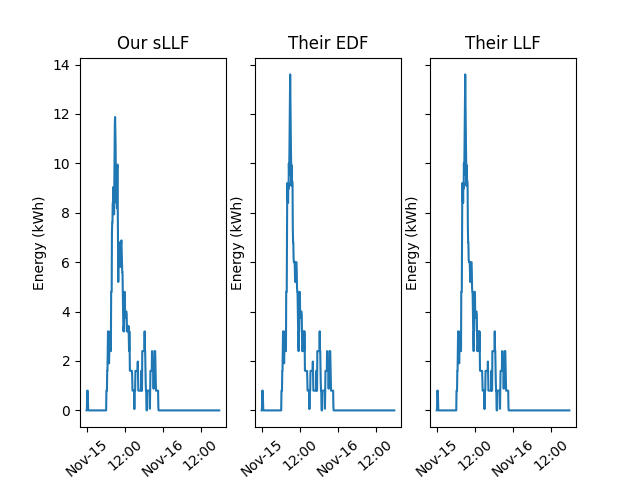
\includegraphics[width=0.8\textwidth]{images/experiments/plot-sLLF-comparison.png}
    \centering
    \caption[Porovnanie ]{}
    \label{acndata:obr}
\end{figure}


% pridat mnozstvo pozadovanej energie tiez?

\begin{table}[H]
    \begin{tabular}{lllll}
    Algoritmus                    &  sLLF & EDF & LLF   & \\
    Pomer dodanej energie (v \%) & 100 & 100  & 100 &   \\
    Množstvo dodanej energie     & 617.73 &  617.73 & 617.73 &  \\
    Cena energie                &  47.14 & 47.08 &  47.08 &   \\
    Poplatok za výkon            & 2210.17 & 2531.23 & 2531.23  &  \\
    Celková cena energie         & 2257.31  & 2578.31 & 2578.31  &  \\
    \$/kWh                       & 3.65 & 4.17 & 4.17 &
    \end{tabular}
\end{table}

    



% \begin{figure}[H]
%     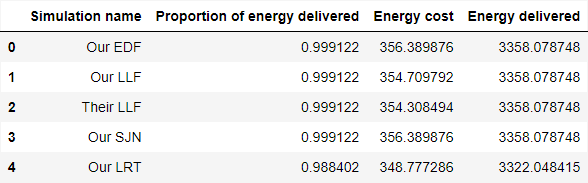
\includegraphics[width=1\textwidth]{images/experiment_comparison.png}
%     \centering
%     \caption[Typy nabíjania elektromobilov]{Tabuľka porovnávajúca výkonnosť (schopnosť dodať čo najviac energie a náklady) rôznych optimalizačných algoritmov s použitím LLF.}
%     \label{typynabijania:obr}
%     \end{figure}



%     \begin{figure}[H]
%         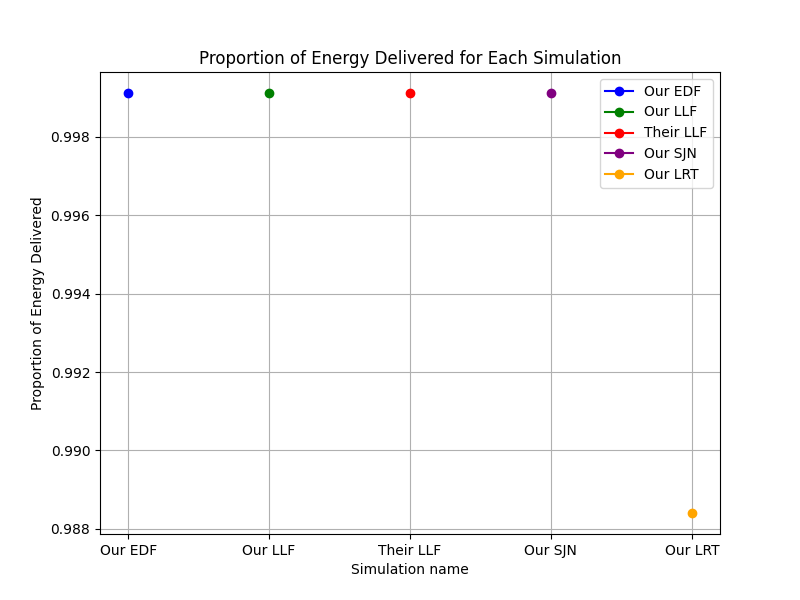
\includegraphics[width=1\textwidth]{images/exp1.png}
%         \centering
%         \caption[Typy nabíjania elektromobilov]{Tabuľka porovnávajúca výkonnosť (schopnosť dodať čo najviac energie a náklady) rôznych optimalizačných algoritmov s použitím LLF.}
%         \label{typynabijania:obr}
%         \end{figure}
    

\section{Druhý experiment}
Cieľom druhého experimentu je porovnať výkonnosť online algoritmov založených na triedení pri riešení formulovaného problému (odkaz).

\subsection{Vstupné dáta}
Vstupné dáta o príchodoch elektromobilov (plugin udalosti) načítavame z nabíjacej stanice Caltech. Ako začiatok príchodov elektromobilov sme nastavili 9. September 2018 a ako koniec príchodov elektromobilov sme nastavili 11. Septembra 2018. Dokopy sme dostali 

\subsection{Nastavenia}
Používame obmedzenia a nabíjačky nabíjacej stanicu Caltech ACN. Pre jednoduchosť sme nastavili, aby nabíjačky boli typu BASICEVSE. Obmedzenia pre nevyváženú trofázovú infraštruktúru siete zostali nezmenené.  Tarify, ktoré používame sa nazývajú $sce\_tou\_ev\_4\_march\_2019$.


\subsection{Výsledky}



% porovnat PPC + sLLF vs PPC + LLF aby sme zistili vysledky stabilnych dodavok nabijania




% \begin{figure}[H]
%     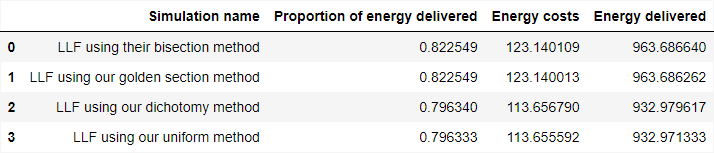
\includegraphics[width=1\textwidth]{images/experiment2_comparison.png}
%     \centering
%     \caption[Typy nabíjania elektromobilov]{Tabuľka porovnávajúca výkonnosť (schopnosť dodať čo najviac energie a náklady) rôznych optimalizačných algoritmov s použitím LLF.}
%     \label{typynabijania:obr}
%     \end{figure}









% TU nieco spomenut co sa tyka vysledkov ich konvergencie





\section{Tretí experiment}




